\chapter{Dataset}
\label{cha:dataset}

Most of the existing SISR methods are trained and evaluated on simulated datasets which assume simple and uniform degradation (i.e., bicubic degradation). Unfortunately, SISR models trained on such simulated datasets are hard to generalize to practical applications since the authentic degradations in real-world LR images are much more complex\cite{cai2019realworld}. Creating a large and varied enough dataset of real-world organic data of paired LR-HR images poses a challenge by itself, that being said the results of this reserch rely heavily on the quality of the data so a lot of work has gone into ensuring that the content of each pair of frames is consistent and reliable without sacrificing too many frames.

The main problems regarding the creation of the LR-HR pairs from two different cameras can be synthetised in:
\begin{itemize}
  \item different lens distortion
  \item spatail alignment
  \item temporal alignment
\end{itemize}

Focal length and Field of View are strongly related one to the other. The Field of View (FOV) describes the physical area of the world that can be imaged on a sensor through a determined lens system, when described in degrees it's referred to as Angular FOV or AFOV.
The focal length of a lens is a fundamental parameter that describes how strongly it focuses or diverges light. A large focal length indicates that light is bent gradually while a short focal length indicates that the light is bent at sharp angles.
The focal length of a lens defines the AFOV, for a given sensor size, the shorter the focal length, the wider the AFOV. Additionally, the shorter the focal length of the lens, the shorter the distance needed to obtain the same FOV compared to a longer focal length lens\cite{flength}.

\begin{figure}[h]
  \centering
  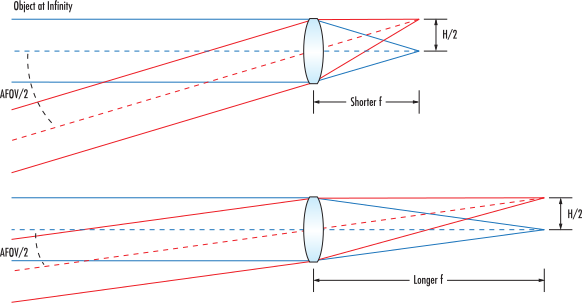
\includegraphics[scale=0.5]{figures/AFOV.png}
  \caption{For a given sensor size H a longer focal length produces a larger AFOV}
\end{figure}

The term distortion is often applied interchangeably with reduced image quality. However, distortion is an individual aberration that does not reduce the information in the image; most aberrations mix information together to create image blur, distortion simply misplaces information geometrically. This means that known distortion can be mapped or calculated and removed from an image, whereas information from other aberrations is lost and cannot easily be recreated.

Distortion is determined by the optical design of the lens. Lenses with larger FOVs will exhibit greater amounts of distortion, larger FOVs (a result of low magnification or short focal length) are more susceptible to distortion than smaller FOVs (high magnification or long focal length). The wide FOVs achieved by short focal length lenses must be weighed against the aberrations introduced to the system (such as distortion)\cite{distortion}.

\begin{figure}[h]
  \centering
  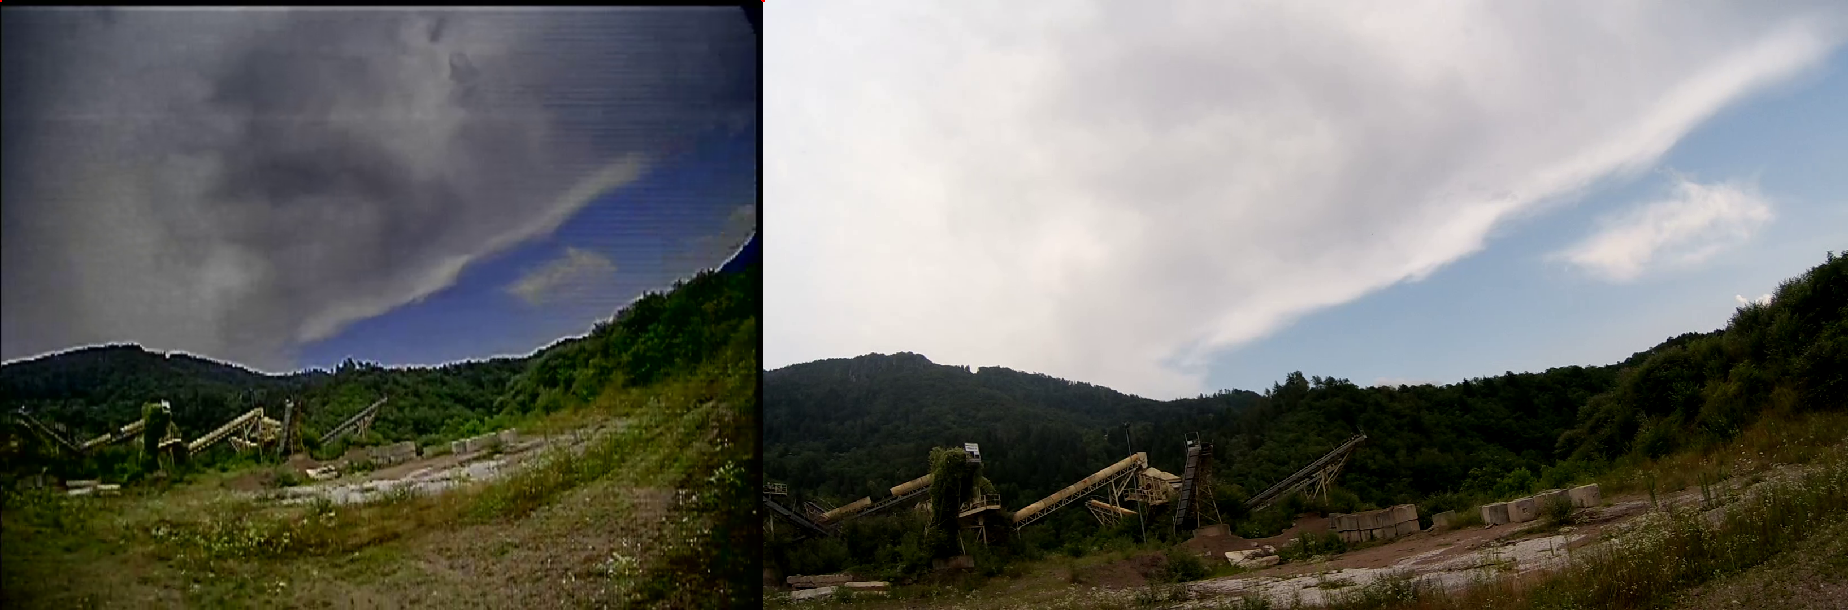
\includegraphics[scale=0.25]{figures/OG_sbs.png}
  \caption{Unprocessed LR and HR frames captured at the same instant}
  \label{img:og_sbs}
\end{figure}

As shown in Figure \ref{img:og_sbs} both images suffer from a great amount of distortion, it's expecially noticiable on the sides of the image. A solution to this problem is to calibrate both cameras and using the obtained information to reproject all the image points without the distortion.

Nevertheless removing the distortion is not enough, it's easy to see how the LR camera, with its shorter focal length and larger AFOV, captures a much larger angular section of the world compared to its HR counterpart, this is a spatial misalignment problem, but not the only couse. As explained previously both cameras are fixed in place, however the entire rig is subject to strong vibrations caused by turbolences, high speed and the four motors spinning at tens of thousands of rounds per minute. All this shaking causes the cameras to move sligthly in all three axis, requiring further work in post processing to get the images aligned.
It's been decided to ignore the parallax error produced by the distance between the cameras. The two sensors sit at approximately \#TODO cm one from another, this causes a sort of "stereo" effect when subjects come close to the camera lenses, however due to the large AFOV this effect is present only at close distances unlike the dataset videos which are almost entirely show subject at several meters of distance, rendering the effect less noticiable or missing completely.\newline

Another notable problem encountered during the dataset processing is temporal alignment. The cameras shoot at 25fps and 60fps with shutter speed of, respectively, 1/50s and 1/120s, the result is that only few frames end up capturing the same instant, with some partially overlapping and others starting at different times.

\begin{figure}[h]
  \centering
  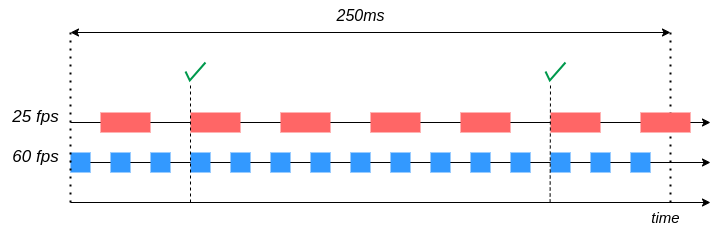
\includegraphics[scale=0.5]{figures/temporal_align.png}
  \caption{How frames are captured over the span of 1/4 of a second}
  \label{img:temp_align}
\end{figure}

As shown in Figure \ref{img:temp_align} only a handful of frames perfectly overlap and start capturing at the same moment. This turned out to be one of the main causes of missed alignment.
How there three problems have been tackled will be discussed in greater detail in chapters \ref{sec:camera_calib}, \ref{sec:temp_align} and \ref{sec:spatial_align}.

\section{Cameras}
\label{sec:cameras}

HR frames have been captured using a Runcam 2\cite{runcam}, the digital camera offers to record at 1920*1440@30, 1080p@60 and 720p@120. To compromise between resolution and frame rate all the HR clips have been recorded in FullHD 1920*1080 at 60 frames per second, although the camera is capable of capuring higher resolution images a lower frame rate would have made difficult to syncronize LR and HR frames resulting in a much lower amount of valid matches.
\begin{figure}[h]
  \centering
  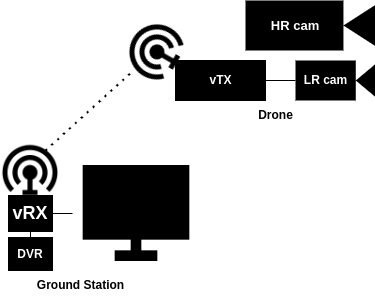
\includegraphics[scale=0.5]{figures/recording_schematics_2.png}
  \caption{Structure of the recording scheme}
\end{figure}
To capture LR frames we used a CADDXFPV Ratel2 Analog Camera\cite{caddx}. As shown in Figure 1.1, the camera is connected to a 5.8Ghz video transmitter (vTX) that streams the signal to a receiver (vRX) on the ground, the receiver is connected the the natigation screen and also to the DVR (Digital Video Recorder) that saves the video stream on an SD card. While the camera itself can capture 1200TVL the colour encoding conversion standard in use is PAL\cite{pal} so accordingly to the standard, once recorded via DVR the rsolution of the video is 720*576 and the frame rate 25 frames per second.

Another mayor difference between the two cameras is the field of view, respectively 120° for the Runcam and 165° for the Ratel2. This is due a a different combination of lens and sensor size, and results in two widely different video streams with a great amount of distortion, before running any kind of training both images must be rectified and the content of each frame must overlap with the one recorded and the other camera.The final results are shown side-by-side in Table \ref{tab:cam_table}.






\begin{table}[h]
\centering
\caption{Resulting video streams}
\label{tab:cam_table}
\begin{tabular}{l|l|l|l|l|}
  \cline{2-5}
                                        & \cellcolor[HTML]{C0C0C0}Resolution {[}px{]} & \cellcolor[HTML]{C0C0C0}Aspect Ratio & \cellcolor[HTML]{C0C0C0}Frame rate {[}fps{]} & \cellcolor[HTML]{C0C0C0}Field of View {[}°{]} \\ \hline
  \multicolumn{1}{|l|}{Runcam 2}        & 1920*1080                                   & 16:9                                 & 60                                           & 120                                           \\ \hline
  \multicolumn{1}{|l|}{CADDXFPV Ratel2} & 720*576                                     & 4:3                                  & 25                                           & 165                                           \\ \hline
  \end{tabular}
\end{table}





\section {Camera Calibration}
\label{sec:camera_calib}

The library OpenCV\cite{opencv} offers a large set of powerful modules for image manipulation and computer vision, among all the others, its pinhole camera model has all the tools to efficiently perform calibration and rectification.

\begin{figure}[h]
  \centering
  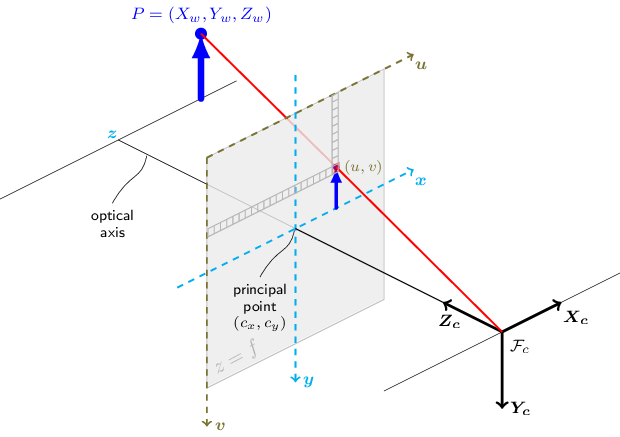
\includegraphics[scale=0.3]{figures/pinhole.png}
  \caption{Illustration of the pinhole camera model}
  \label{img:pinhole_img}
\end{figure}

The pinhole camera model describes the mathematical relationship between the coordinates of a point in three-dimensional space and its projection onto the image plane of an ideal pinhole camera, where the camera aperture is described as a point and no lenses are used to focus light\cite{wikipinhole}.
The distortion-free projective transformation given by a pinhole camera model is shown below.

\[s \; p = A \begin{bmatrix} R|t \end{bmatrix} P_w,\]

Where \(P_w\) is a 3D point expressed with respect to the world coordinate system, \(p\) is a 2D pixel in the image plane, \(A\) is the camera intrinsic matrix, \(R\) and \(t\) are the rotation and translation that describe the change of coordinates from world to camera coordinate systems (or camera frame) and \(s\) is the projective transformation's arbitrary scaling and not part of the camera model\cite{opencvcalib}.

The camera intrinsic matrix \(A\) (Figure \ref{fig:camera_matrix}) projects 3D points given in the camera coordinate system to 2D pixel coordinates, it's composed of the focal lengths \(fx\) and \(fy\), which are expressed in pixel units, and the principal point (\(cx\),\(cy\)), that is usually close to the image center\cite{opencvcalib}\cite{888718}.

\begin{figure}[h]
\caption{Intrinsic camera matrix}
\label{fig:camera_matrix}
\[A = \left (
  \begin{array}{ c c c}
  f_x & 0   & c_x \\
   0  & f_y & c_y \\
   0  & 0   & 1 \\
  \end{array}
\right )\]
\end{figure}


The intrinsic camera matrix is not the only set of parameters estimated during the calibration process. Real lenses introduce, to some degree, barrel distortion and tangential distortion, to compensante for this, a vector of distortion coefficents is estimated along the intrinsic camera matrix and subsequently used in all the applications of the model.\newline


The estimation algorithm is based on \cite{888718} and \cite{matlab}, several pictures of a calibration pattern of known geometry are taken from different positions, for each view of the pattern the algorithm computes the intrinsic parameters, after that the camera position in respect to the calibration pattern is estimated using solvePnP\cite{opencvsolvepnp}. The last step is to run the Levenberg-Marquardt optimization algorithm to minimize the reprojection error (sum of the square distances between the observed features on the calibration pattern and the estimated position of said feature reprojecting the 3D object point on the visual plane).

Most of the time a chessboard pattern is enough to perform this kind of calibrate, however OpenCV's findChessboardCorners \#TODO function only detects the pattern when the entire board is in frame, this means that the detection fails most of the times when the board is moved to the corners of the screen, which is exactly where the distortion is more pronounced. For this reason a ChArUco board has been used insted.

\begin{figure}[h]
  \centering
  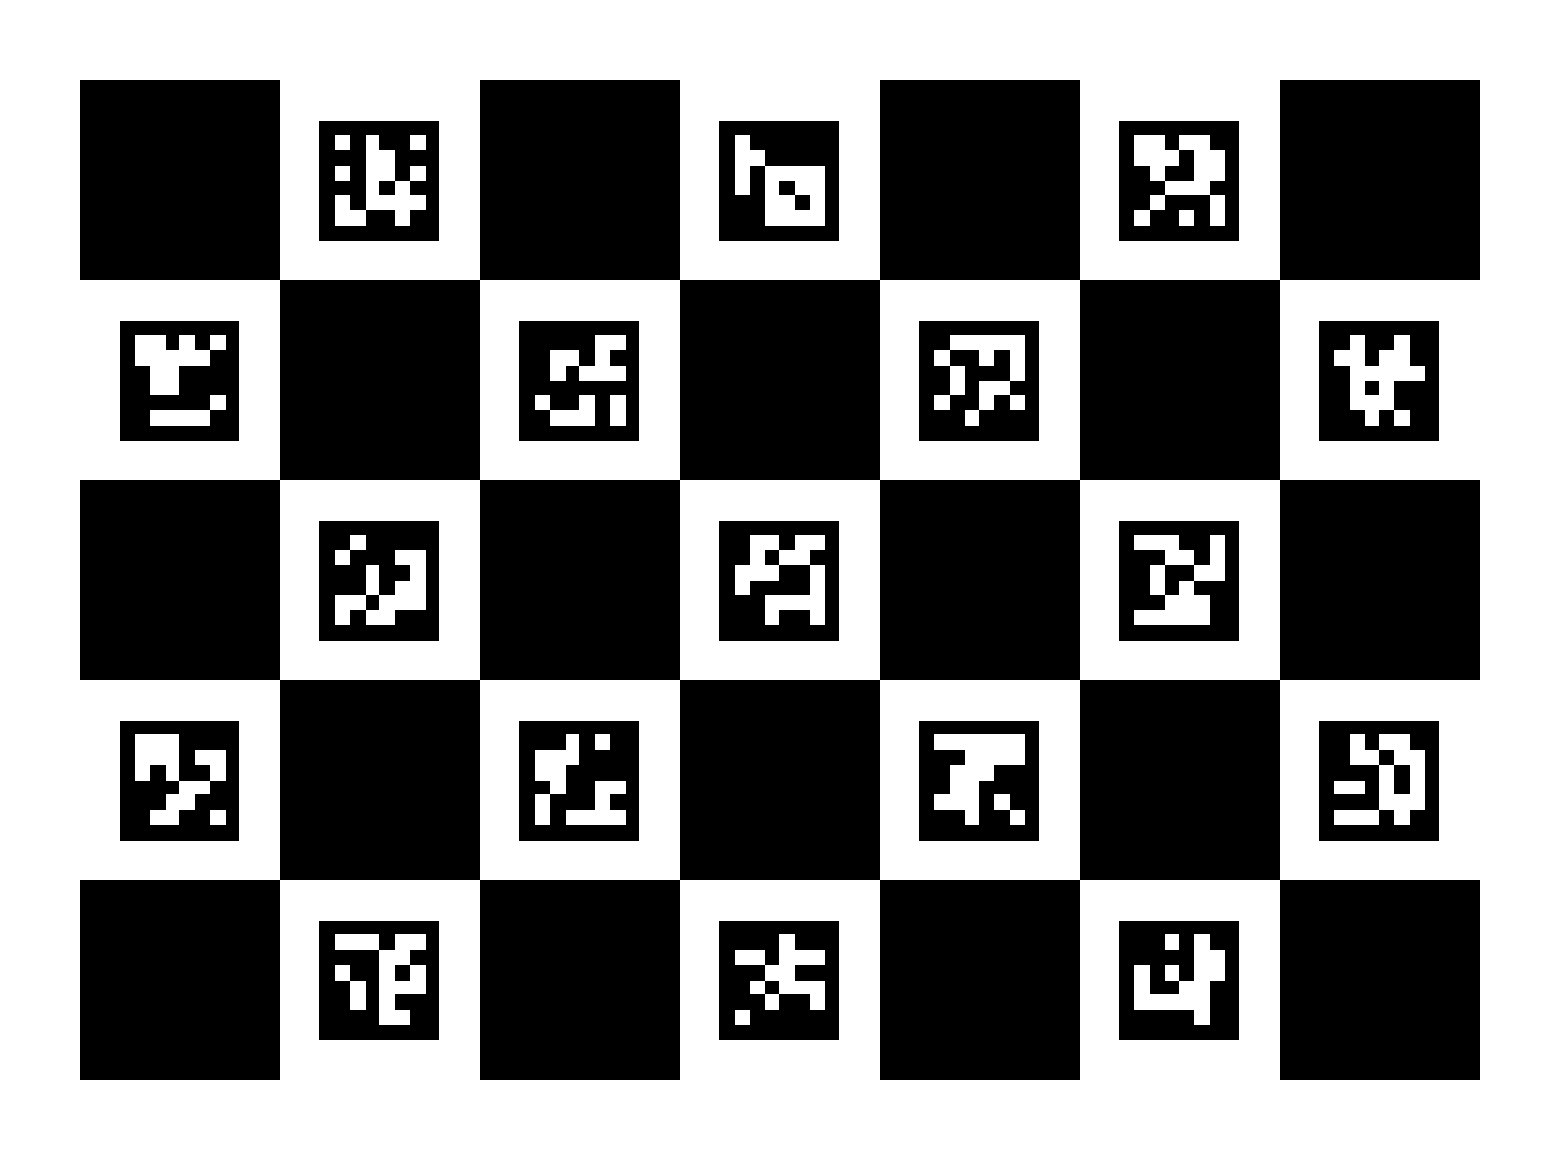
\includegraphics[scale=0.15]{figures/charucoboard.png}
  \caption{ChArUco board used for the calibrations}
  \label{img:ch_board}
\end{figure}

The ChArUco board (Figure \ref{img:ch_board}) incorporates a standard chessboard pattern with a set of ArUco markers for detection, this allows the algorithm to detect the unique labels and from that it extrapolates the exact position of each pattern corner even if the board is only partially in frame. Each pattern corner is firsly refined at sub-pixel level for better accuracy, and after that all the detected corners are paired, as 2D coordinate, to the 3D points in the calibration pattern frame of reference.

The quality of the board used for calibration is extremely important for proper parameter estimation, paper or plastic boards can introduce imperceptible deformations that can seriously tarnish the results of the process, on top of that temperature or humidity changes can cause the board to contract or dilate, thus a flat tv screen has been used to run the calibration for both camera, ensuring a levelled plane and uniform illumination on the entire surface. Another reson to choose a big tv screen over a printed pattern is that the low resolution of the LR camera makes the detection of the ArUco markers difficult, resulting in very close up videos with mediocre results.

\begin{figure}[h]
  \centering
  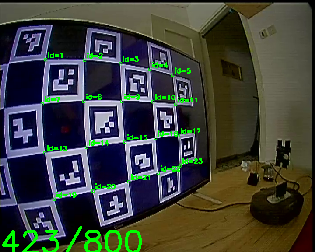
\includegraphics[scale=0.7]{figures/not_all.png}
  \caption{Frame taken during the calibration process. It shows how, even if the pattern is only partially visible, the corners are succesfully detected and labeled with the correct ID.}
  \label{img:ch_calib}
\end{figure}

To ensure pecise calibration results a flat pattern is appropriate, but not enough. The algorithm needs hundreds of data points over the span of tenths of images, it's importand to make sure that the images cover a large volume of angles w.r.t the target and ideally that they are distrubuted uniformally in the set. In order to follow these constraints closely and to keep the process as repeatable as possible without making it too time consuming, the calibration pipeline has been divided in two parts that can be run together: datapoints capture and intrinsic parameters estimation.

During the datapoints capture, to the script is fed video a taken from one of the two cameras, panning around the calibration pattern, slowly to avoid vibrations and motion blur and progressevely covering all the camera frame from various angles and distances. A frame is considered valid when the numbers of detected corners is higher than a threshold set in advance, this is to make sure that even when part of the board is not visible (i.e. around the corners) data is collected but if too few corners are detected (i.e. due to sudden movements or distance) the data is considered bad and the  frame discarded.

Once enough valid frames have been captured a number of those data points is randomly sampled from the pool and fed to camera calibration function that calculates the intrinsic camera matrix and the distortion coefficents vector. As hinted in the chapter introduction this kind of calibration is an optimization problem, in particular the optimizer tries to minimize the RMS reprojection error, which is the distance of the pattern keypoints detected on the image and the same points reprojected on the image using the calibrated camera model. This distance is expressed in pixels and typically one should expect to get values around 1.

A larger amount of images does not necessarily mean a better result and also the level of the threshold has a big an impact on the quality of the calibration, it's a tradeoff between giving the algorithm more datapoints around the frame edges and dropping points that might affect negatively the process.

\begin{figure}[H]
  \centering
  \begin{subfigure}{.5\textwidth}
    \centering
    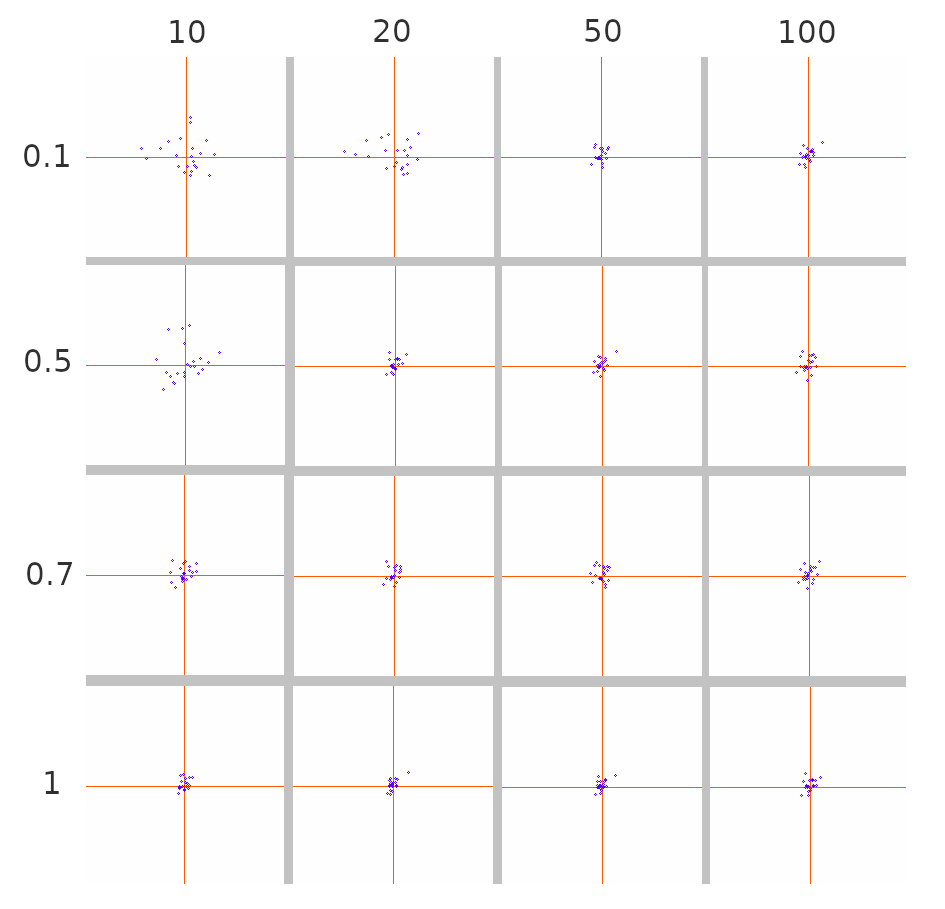
\includegraphics[width=.8\linewidth]{figures/reprj_dist_LR.png}
    \caption{Distrubution of reprojection errors w.r.t. \newline number of samples and threshold.}
    \label{fig:reprj_dist_LR}
  \end{subfigure}%
  \begin{subfigure}{.5\textwidth}
    \centering
    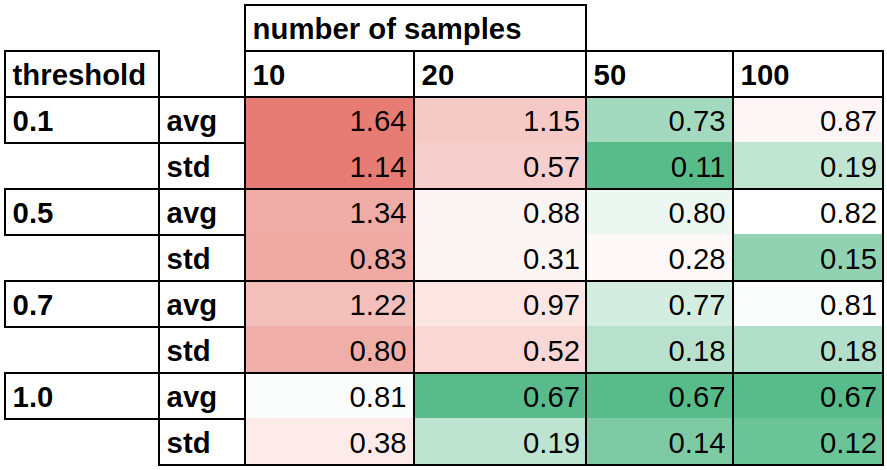
\includegraphics[width=1\linewidth]{figures/calib_results_table_LR.png}
    \caption{RMS reprojection error averaged over 20 calibrations and standard deviation w.r.t. number of samples and threshold.}
    \label{fig:calib_stats_LR}
  \end{subfigure}
  \caption{Analysis of the calibration results with the LR camera.}
  \label{fig:calib_analysis_LR}
\end{figure}

\begin{figure}[H]
  \centering
  \begin{subfigure}{.5\textwidth}
    \centering
    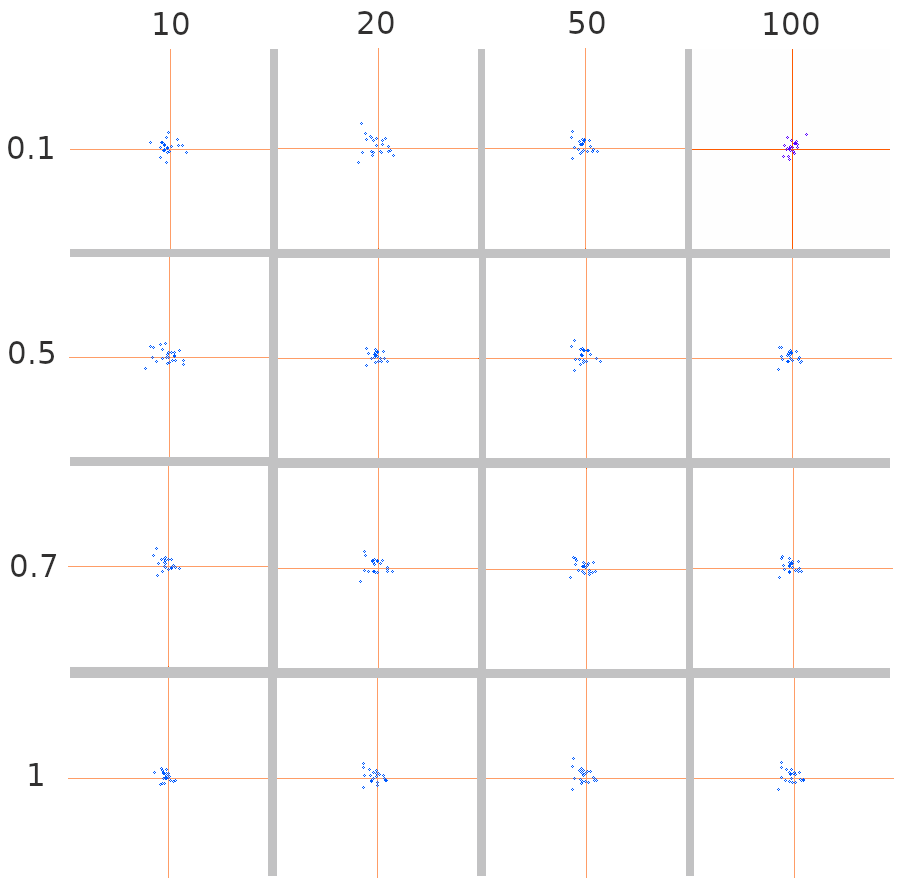
\includegraphics[width=.8\linewidth]{figures/reprj_dist_HR.png}
    \caption{Distrubution of reprojection errors w.r.t. \newline number of samples and threshold.}
    \label{fig:reprj_dist_HR}
  \end{subfigure}%
  \begin{subfigure}{.5\textwidth}
    \centering
    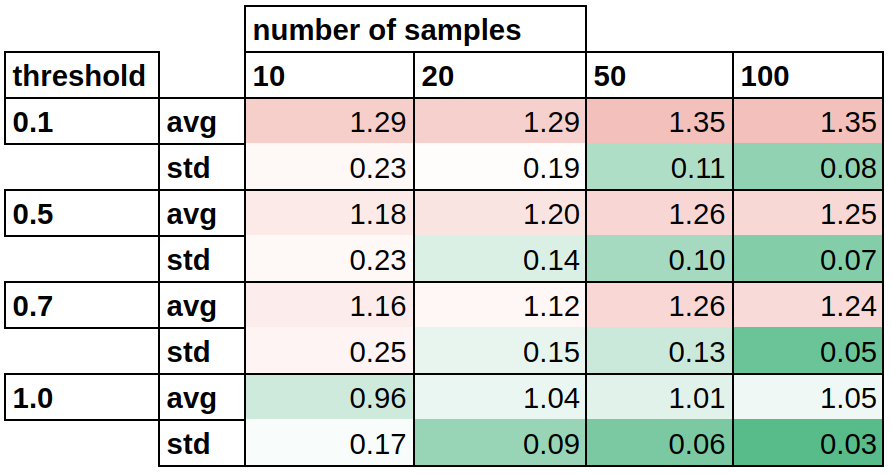
\includegraphics[width=1\linewidth]{figures/calib_results_table_HR.png}
    \caption{RMS reprojection error averaged over 20 calibrations and standard deviation w.r.t. number of samples and threshold.}
    \label{fig:calib_stats_HR}
  \end{subfigure}
  \caption{Analysis of the calibration results with the HR camera.}
  \label{fig:calib_analysis_HR}
\end{figure}
The analysis in Figures \ref{fig:calib_analysis_LR} and \ref{fig:calib_analysis_HR} have been done separately for the low-res camera and the high-res camera. For consistecy it's been used a single video from each camera and a total of around 600 calibrations have been run before averagin for each combination of threshold and amount of frames used.

Figure \ref{fig:calib_stats_LR} and Figure \ref{fig:calib_stats_HR} show how, for both cameras, there's a strong correlation between the number of samples used in each calibration and the consistecy of the inaccuracies, as the standard deviation shrinks with the amount of datapoints. The averaged error doesn't always follow the same pattern, however it's safe to assume that if it doesn't flactuate excessively, a larger set of corners guarantees a better generalization of the camera model. Also, higher thresholds generally yield better results as single frames contain more correlated points, unfortunately this leads to less information about the distortion around the edges of the image to be examined. Generally, a low error on a higher threshold can be misleading as it indicates that the approximation of the camera model is good taking in consideration mostly images that fit inside the entire frame, so around the middle where distortion is present the least.

A second factor to take into consideration is the distrubution of errors, RMS reprojection error only gives information about the averaged distance between detected and reprojected points without taking into account their direction. Figures \ref{fig:reprj_dist_LR} and \ref{fig:reprj_dist_HR} show how for each combination of threshold and number of samples the reprojected points differ from their detected position on the two axis, a good calibration will show a cloud of datapoints distrubuted uniformally aroud the origin, if the spread it skewed in one direction that might be the symptom of a poor estimation or bad measurements. It's worth mentioning that this kind of off-center patterns are not evident from the RMS error reading alone so it's good practice to run a specific check for these particular occurences.

\section{Temporal Alignment}
\label{sec:temp_align}

\section{Spatial Alignment}
\label{sec:spatial_align}
\subsection {Feature Matching}
\label{subsec:feature_match}
\subsection {Template Matching}
\label{subsec:template_match}
